\subsection{SIR Model}

For testing and data generation we have implemented a SIR Model using Python. The code can be found in the given Github repository.\newline
An example of a early model state is shown in Figure~\ref{fig:1}

\begin{figure}[H]
	\centering
	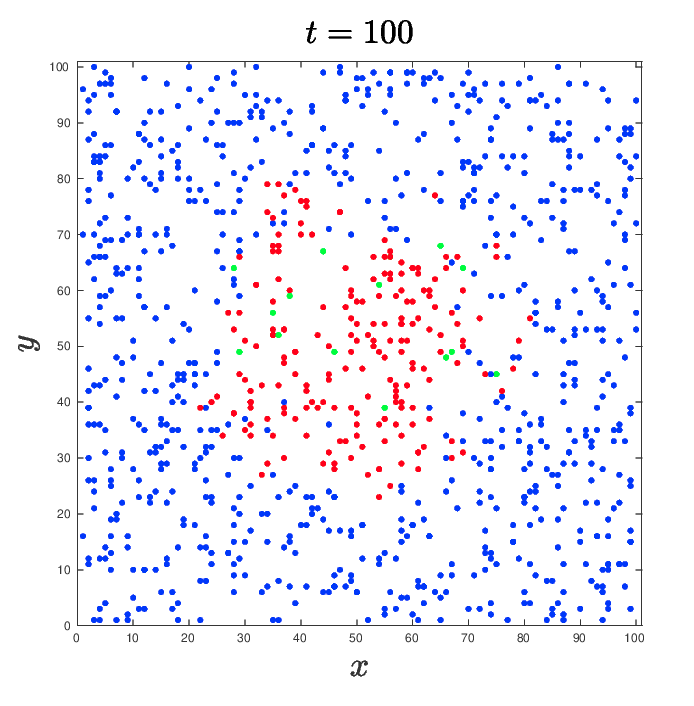
\includegraphics[width=0.4\linewidth]{initial_setup.png}
	\caption{Early state of SIR model, blue dots = susceptibles, red dots = infected agents, green dots = Recovered agents}%
	\label{fig:1}
\end{figure}

In this case, 1000 agents were initialized on a 100 by 100 grid, where a certain amount of infected agents were introduced as a seed. Letting the agents perform random walks on the grid (maximally one step each time step with probability $d$), and letting the model converge, the results in figure~\ref{fig:2} can be observed.

\begin{figure}[H]
	\centering
	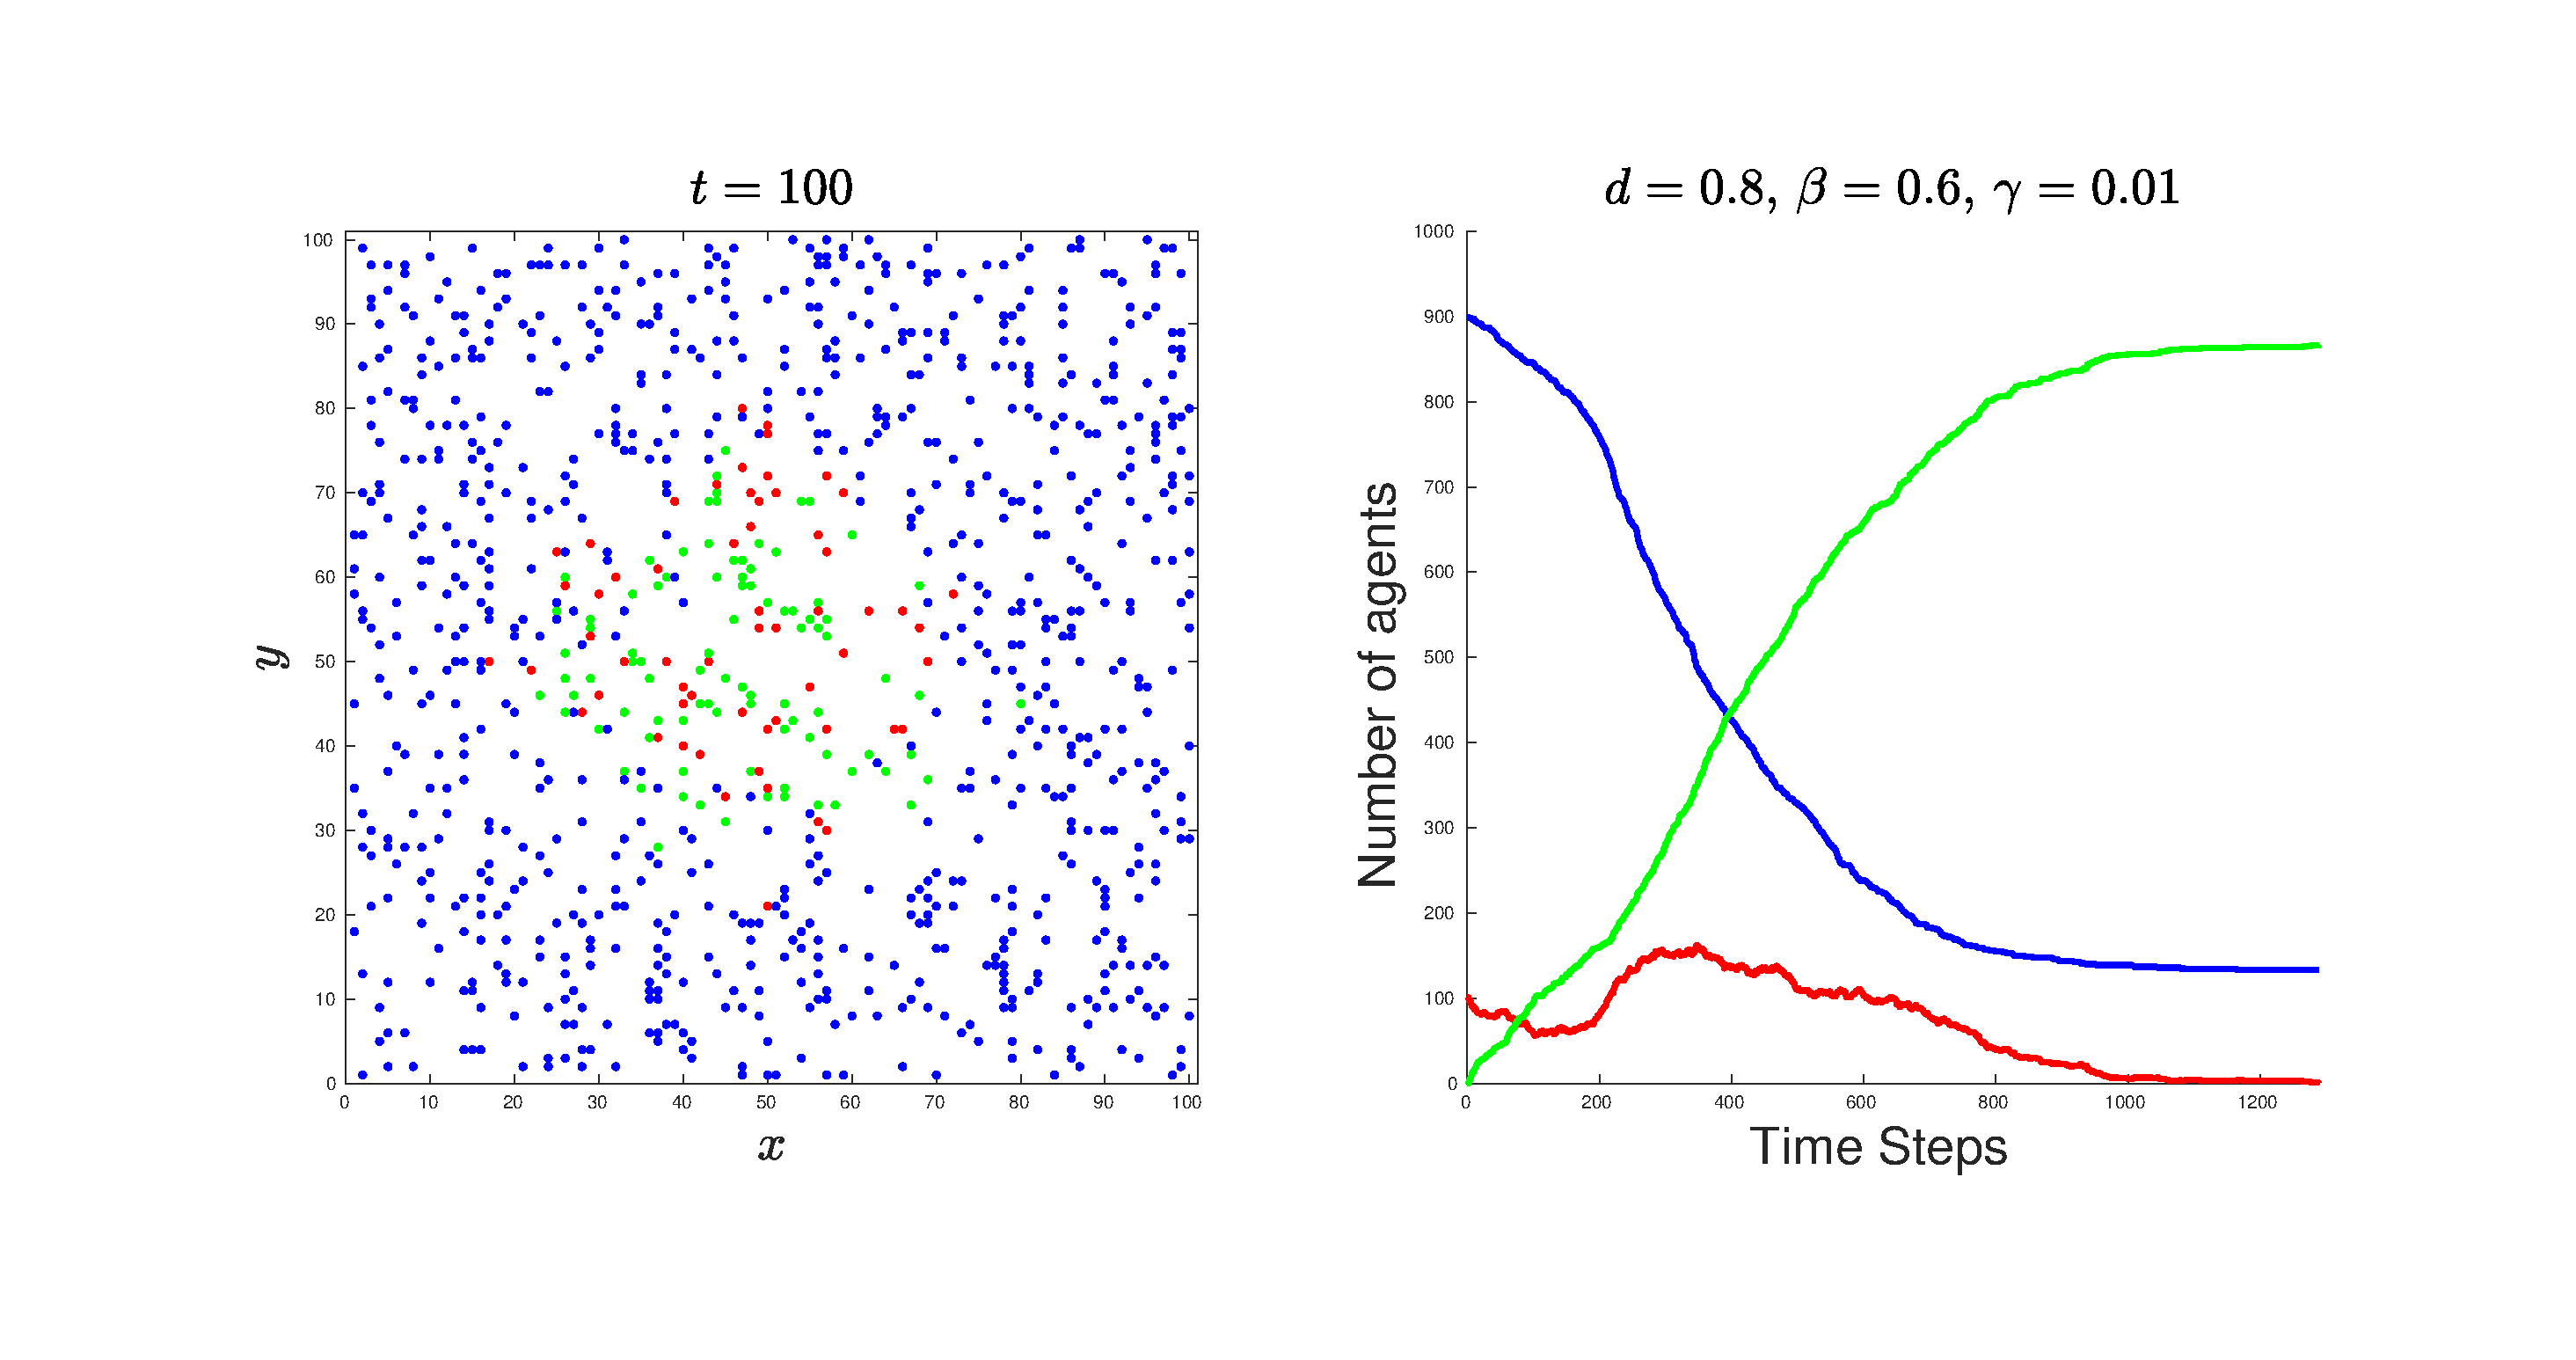
\includegraphics[width=0.9\linewidth]{1_1000_agents}
	\caption{Plot of the proportions of susceptible (blue), infected (red) and recovered (green) individuals in each state over time.}%
	\label{fig:2}
\end{figure}

With the above stated parameters ($d=0.8$, $\beta=0.6$, $\gamma=0.01$), the disease does not spread over the whole population. However over 80\% were infected over time, which could be a very likely scenario of the corona out brake.


\subsection{Improving the Simulation}
Random walk is commonly used for simple Simulations. However this movement pattern does not represent the daily routine of the majority of citizens. It  is more likely that the major part of the population moves around their hometown and travel small distances which leads to clustering of the whole population. To improve the simulation the agents are split into two groups. One group moves random walk like. This group represents e.g. service providers and delivery services. The other group moves around given points. This movement is implemented using polar coordinates with random radius and random angle. The movement pattern of the two groups is illustrated in figure \ref{fig:movementPattern}. 
\begin{figure}[H]
	\centering
	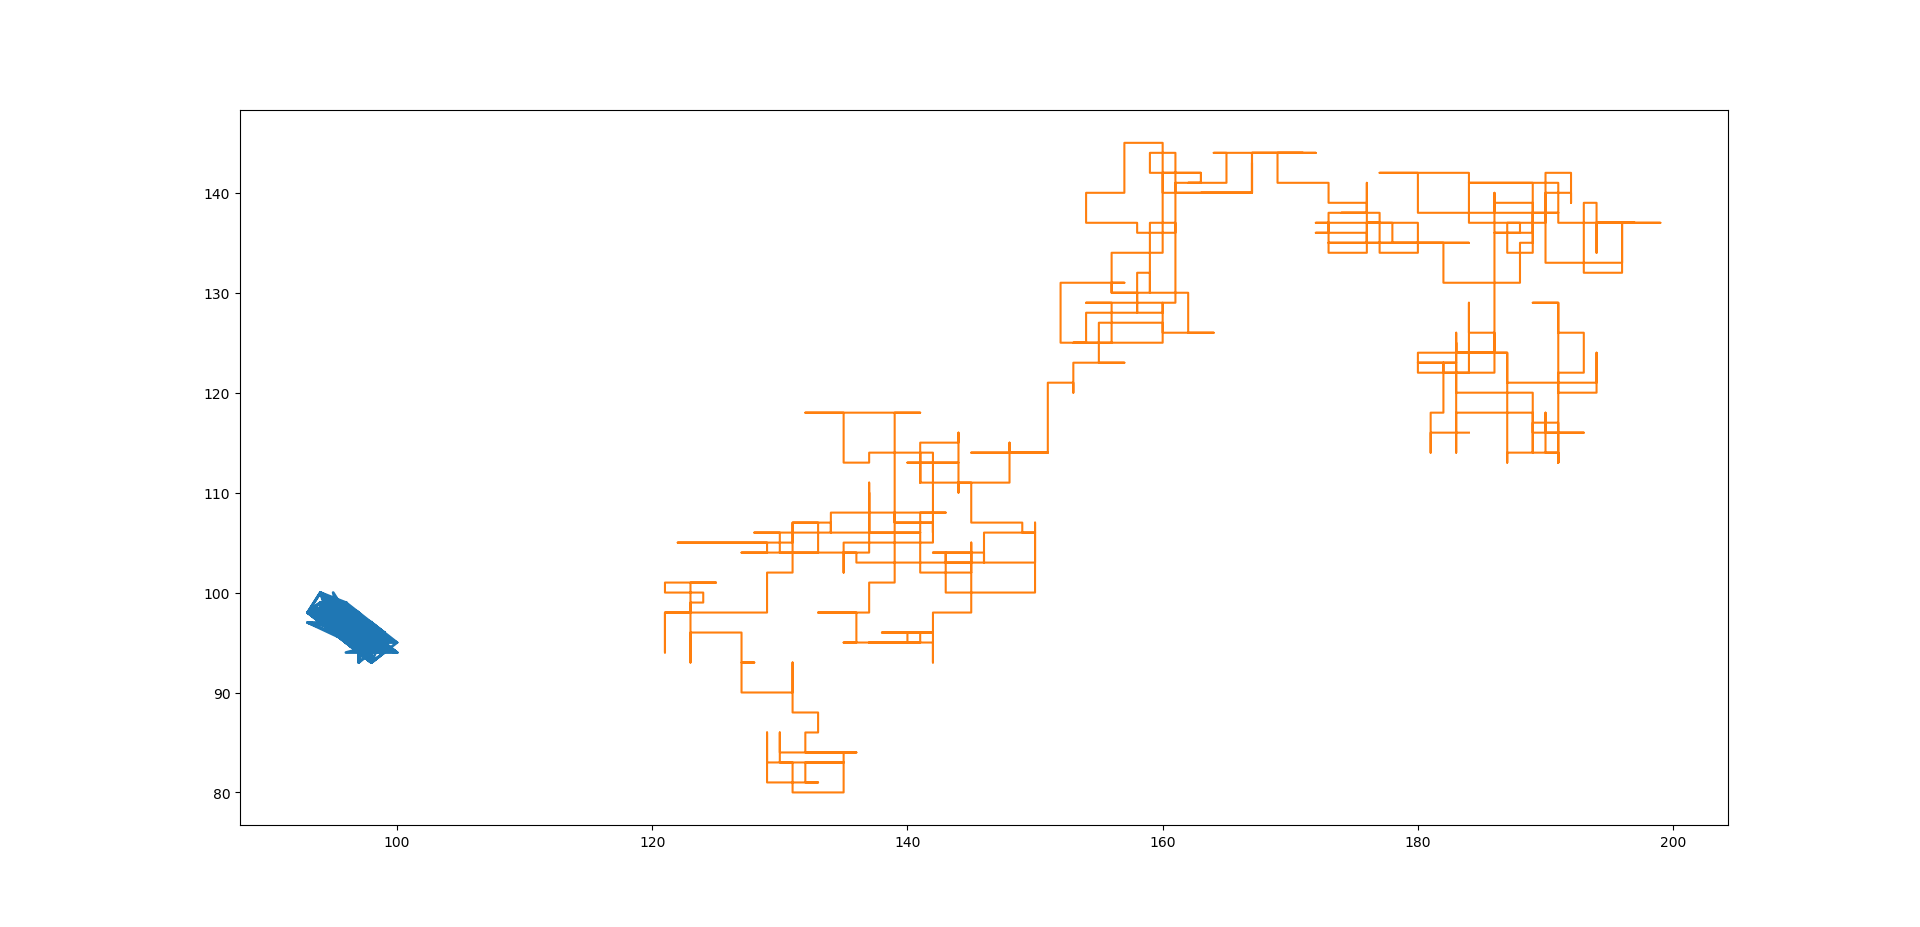
\includegraphics[width=0.9\linewidth]{img/movementPattern.png}
	\caption{Movement pattern of the two groups. Random walk (orange) and localized movement (blue)}%
	\label{fig:movementPattern}
\end{figure}

With these two groups new features like multiple outbreaks of the waves in different clusters can be observed. An example of the improved model is shown in figure \ref{fig:multipleOutbreaks}. In this case 3000 agents were initialized on a 200 by 200 grid with the infection parameters $\beta=0.6$ and $\gamma = 0.01$. $70\%$ of the agents move in clusters. The infection waves at $t = 40$, $t = 210$ and $t= 650$ can be explained by the infection of a new cluster. The second infection wave is illustrated in figure \ref{fig:clusterInfection}. The whole simulation can be found  as Video \url{https://youtu.be/c7ehtN-1n9w}.

\begin{figure}[H]
	\centering
	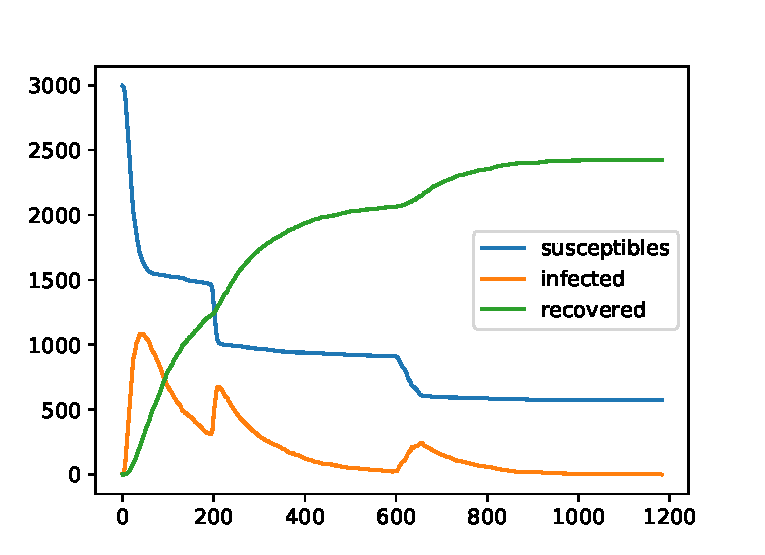
\includegraphics[width=0.7\linewidth]{img/multipleOutbreaks.pdf}
	\caption{Plot  of  the  proportions  of  susceptible  (blue),  infected  (orange)  and  recovered  (green)  individuals  in  each  state over time.)}%
	\label{fig:multipleOutbreaks}
\end{figure}

\begin{figure}[H]
    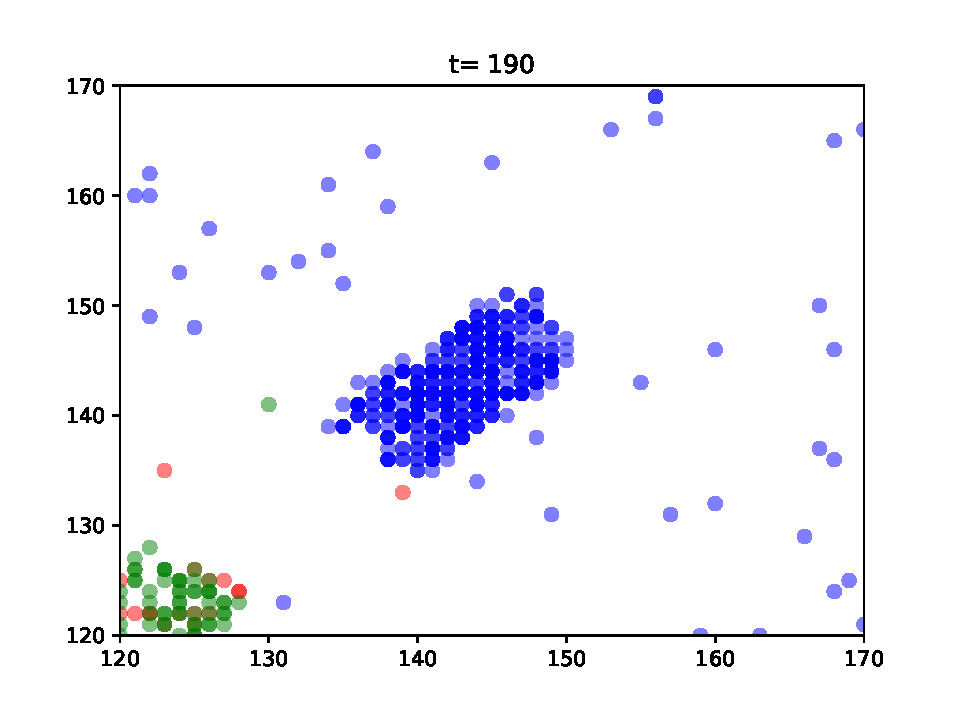
\includegraphics[width=.24\textwidth]{img/cluster190.pdf}\hfill
    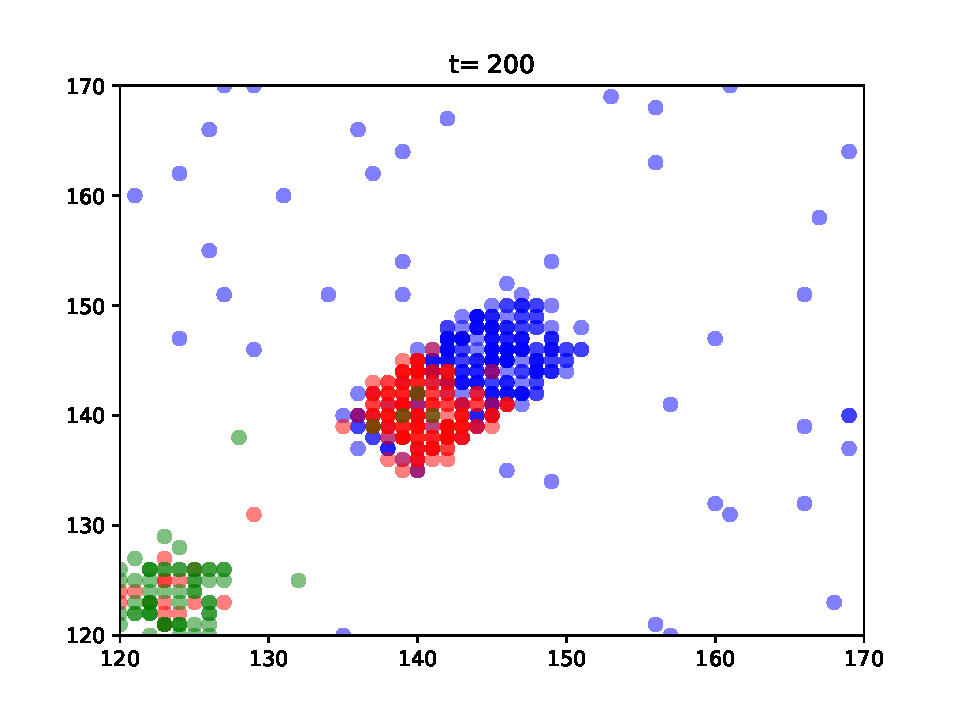
\includegraphics[width=.24\textwidth]{img/cluster200.pdf}\hfill
    \\[\smallskipamount]
    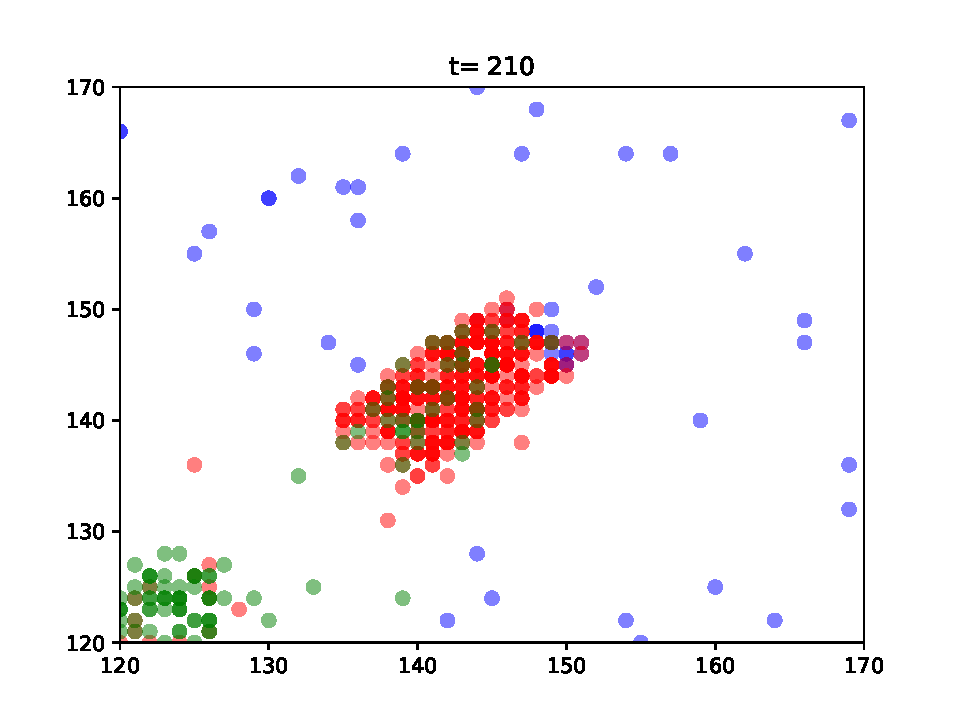
\includegraphics[width=.24\textwidth]{img/cluster210.pdf}\hfill
    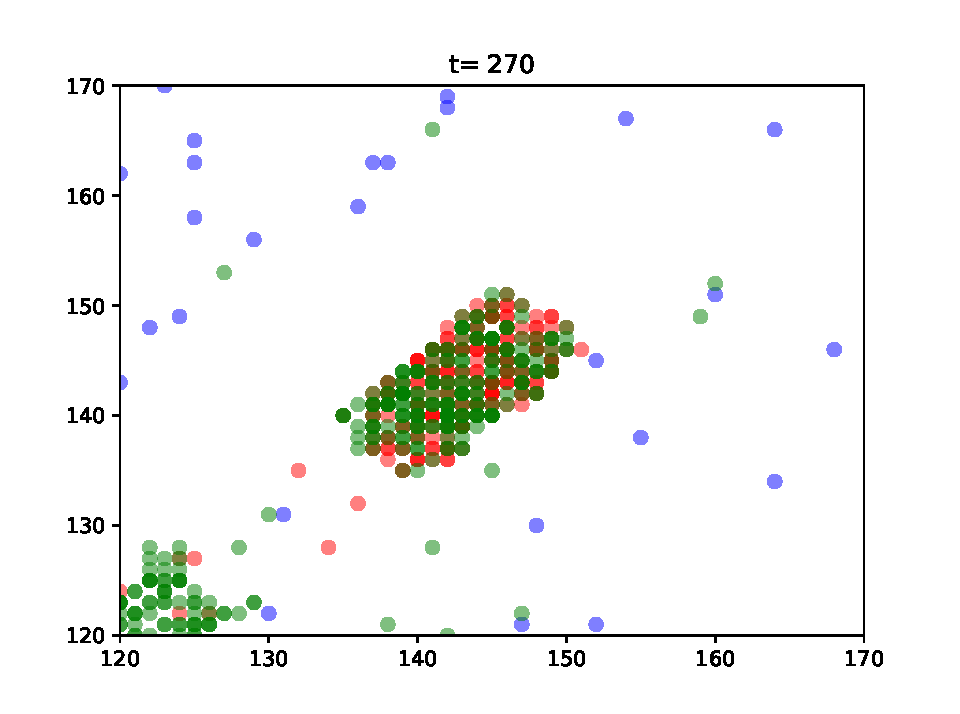
\includegraphics[width=.24\textwidth]{img/cluster270.pdf}\hfill
    \caption{Second infection waves in figure~\ref{fig:multipleOutbreaks}. Blue: not infected, red: infected, green: recovered. $t = 190$ cluster gets infected (top left), $t = 200$ disease spreads (top right ), $t = 210$ most of the cluster is infected (bottom left) and $t = 270$ cluster recovers (bottom right).}%
    \label{fig:clusterInfection}
    
\end{figure}